\chapter{Appendix: Supplementary Material}
\label{appendix:supplementary}

\section{Additional Results}

\textbf{Quantitative Comparison Against Zero123++.} Many state-of-the-art text-to-3D methods utilize a two-stage pipeline: first generating multi-view images, then performing sparse-view 3D reconstruction. Our work enhances the first stage and is compatible with various reconstruction methods. Here we quantitatively compare our method to Zero123++~\cite{shi2023zero123singleimageconsistent}, a widely-used multi-view generation model.

We generated results using prompts from the Objaverse test set. For our method, we first produced coarse objects using Shap-E and refined them using Sharp-It. For Zero123++, we conditioned the generation on images produced from the same prompts. We measured FID and CLIP similarity between input text prompts and resulting images. Results in Table~\ref{tab:quant-zero123} demonstrate that our method outperforms Zero123++ in terms of visual quality (FID), while maintaining comparable semantic alignment (CLIP).

\begin{table}[h]
\centering
\caption{Quantitative comparison of our method with Zero123++.}
\begin{tabular}{c c c}
    \hline
    Method          & FID ($\downarrow$) & CLIP ($\uparrow$)  \\
    \hline
    Zero123++       & 51.95              & 0.262\\
    Sharp-It (ours) & \textbf{38.14}     & \textbf{0.264} \\
    \hline
\end{tabular}
\label{tab:quant-zero123}
\end{table}
\begin{figure}[h]
\setlength{\tabcolsep}{1pt}
\begin{tabular}{cccc}
    3DAdapter & Ours & 3DAdapter & Ours \\
    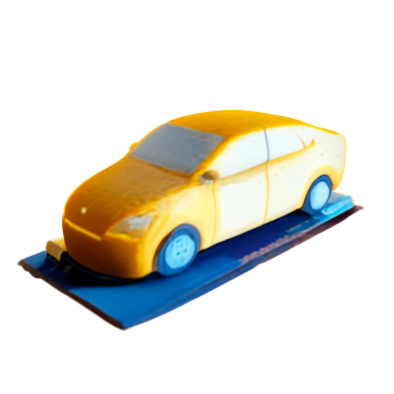
\includegraphics[width=0.25\linewidth]{images/rebuttal/3dadapter_comparison/car_cheese_3dadapter.png} &
    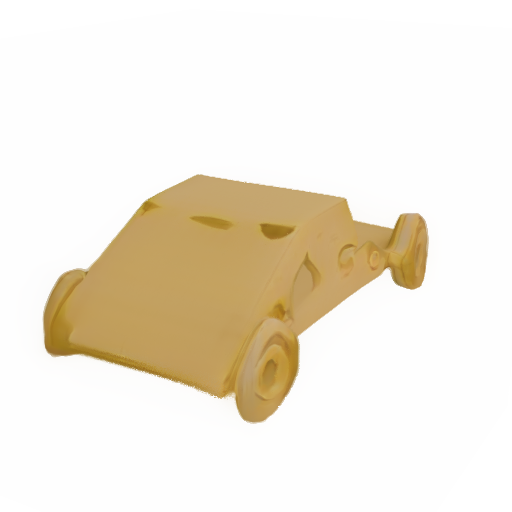
\includegraphics[width=0.25\linewidth]{images/rebuttal/3dadapter_comparison/cheese_car_000.png} &
    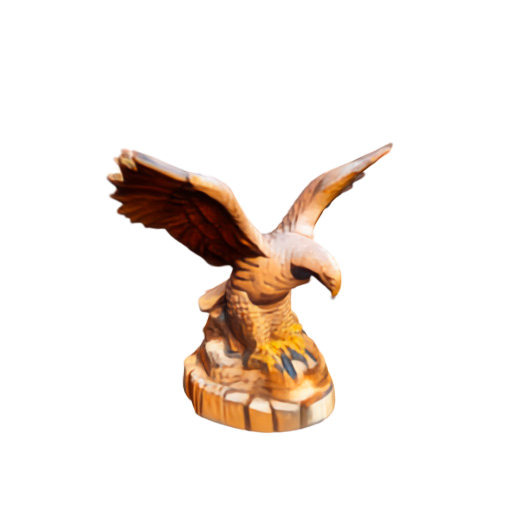
\includegraphics[width=0.25\linewidth]{images/rebuttal/3dadapter_comparison/eagle_3dadapter.png} &
    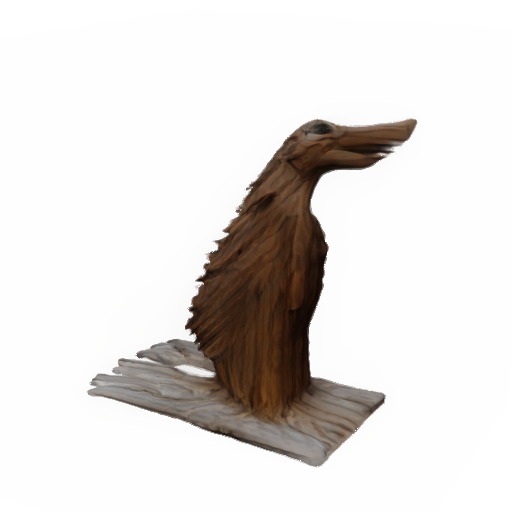
\includegraphics[width=0.25\linewidth]{images/rebuttal/3dadapter_comparison/wood_bald_eagle_000.png} \\
    \multicolumn{2}{c}{``A car made out} & \multicolumn{2}{c}{``A bald eagle car-} \\
    \multicolumn{2}{c}{of cheese''} & \multicolumn{2}{c}{ved out of wood''} 
\end{tabular}
\caption{Comparison of Sharp-Its results against a competing method, 3DAdapter}
\end{figure}
\textbf{Comparison Against 3D-Adapter.} In Figure~\ref{fig:comparison_3d_adapter}, we qualitatively compare our approach against 3D-Adapter~\cite{3dadapter2024}, a recent alternative that directly generates 3D content without intermediate multi-view synthesis.
\textbf{Sharp-It Reliance on Shap-E.} Sharp-It depends on Shap-E's initial coarse outputs. To objectively evaluate enhancement capabilities, our main evaluation used Objaverse objects encoded into Shap-E latent representations. Additional examples illustrating the encoding and subsequent refinement using Sharp-It are shown in Figure~\ref{fig:supp_comparisons}.

\begin{figure}
    \centering
    \setlength{\tabcolsep}{1pt}
    {\small
    \begin{tabular}{cccc}
        \multicolumn{2}{c}{Input (Shap-E)} & \multicolumn{2}{c}{Sharp-It} \\
        % View 1 & View 2  & View 1 & View 2 \\
        %
    
        \multicolumn{1}{c}{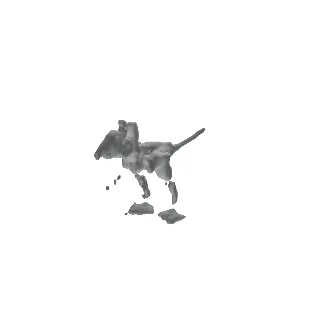
\includegraphics[width=0.24\linewidth, trim=50 0 50 0, clip]{images/supplementary/failure_cases/dino-shap-e-1.png}} &
        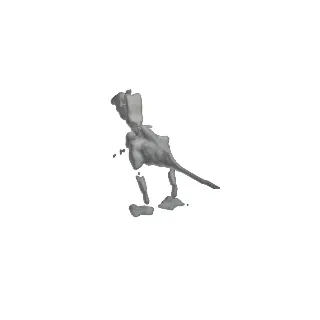
\includegraphics[width=0.24\linewidth, trim=50 0 50 0, clip]{images/supplementary/failure_cases/dino-shap-e-2.png} &
        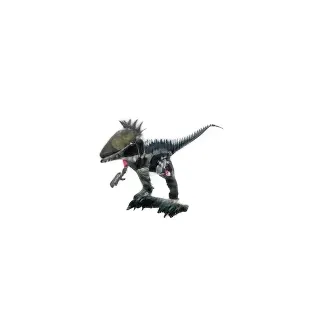
\includegraphics[width=0.24\linewidth, trim=50 0 50 0, clip]{images/supplementary/failure_cases/dino-sharp-it-1.png} &
        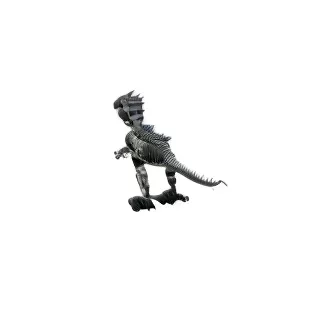
\includegraphics[width=0.24\linewidth, trim=50 0 50 0, clip]{images/supplementary/failure_cases/dino-sharp-it-2.png} \\
        %
        \multicolumn{4}{c}{``A dinosaur''} \\
        %
        \multicolumn{1}{c}{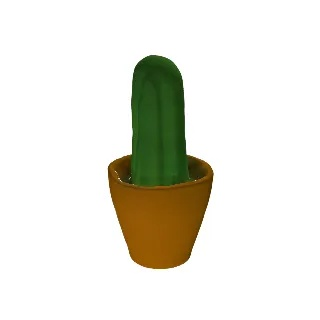
\includegraphics[width=0.24\linewidth, trim=50 0 50 0, clip]{images/supplementary/failure_cases/image-16_r1c1.jpg}} &
        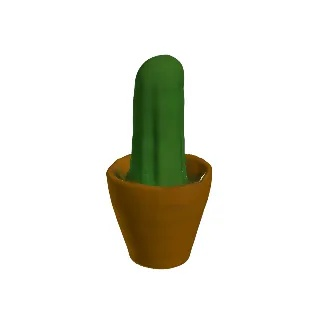
\includegraphics[width=0.24\linewidth, trim=50 0 50 0, clip]{images/supplementary/failure_cases/image-16_r2c1.jpg} &
        
\includegraphics[width=0.24\linewidth, trim=50 0 50 0, clip]{images/supplementary/failure_cases/image-15_r1c1.jpg} &
        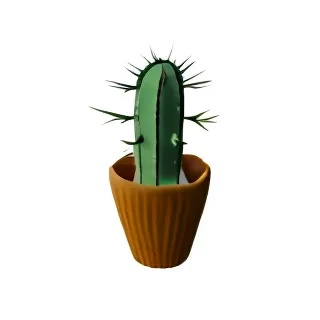
\includegraphics[width=0.24\linewidth, trim=50 0 50 0, clip]{images/supplementary/failure_cases/image-15_r2c1.jpg} \\
        %
        \multicolumn{4}{c}{``A cactus''} \\
        %
        \multicolumn{1}{c}{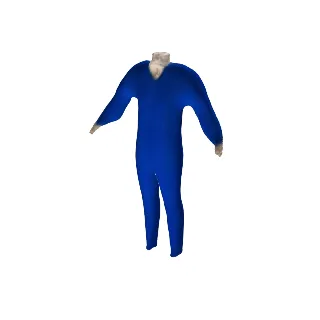
\includegraphics[width=0.24\linewidth, trim=50 0 50 0, clip]{images/supplementary/failure_cases/suit-shap-e-1.png}} &
        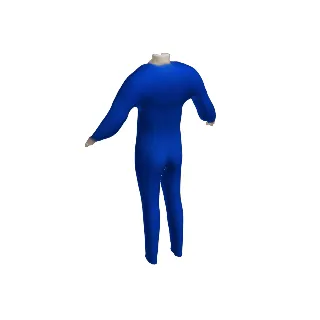
\includegraphics[width=0.24\linewidth, trim=50 0 50 0, clip]{images/supplementary/failure_cases/suit-shap-e-2.png} &
        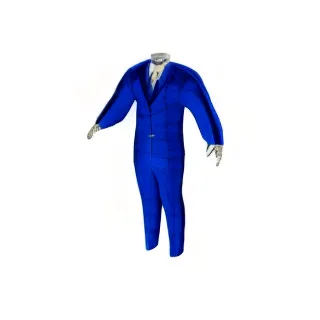
\includegraphics[width=0.24\linewidth, trim=50 0 50 0, clip]{images/supplementary/failure_cases/suit-sharp-it-1.png} &
        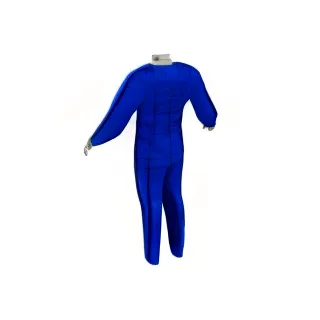
\includegraphics[width=0.24\linewidth, trim=50 0 50 0, clip]{images/supplementary/failure_cases/suit-sharp-it-2.png} \\
        %
        \multicolumn{4}{c}{``A suit''}
    \end{tabular}
    }
    \caption{Refinement results of Sharp-It, Resulting from Shap-E Generation.}
    \label{fig:supp-comparison}
\end{figure}


\section{Failure Cases}

We present failure cases of our method in Figure~\ref{fig:failure_case}. These typically arise from particularly challenging geometry or complex textures in the initial shape provided by Shap-E.

\begin{figure}[h]
\setlength{\tabcolsep}{1pt}
\begin{tabular}{cccc}
     \multicolumn{2}{c}{Shap-E} & \multicolumn{2}{c}{Sharp-It} \\
    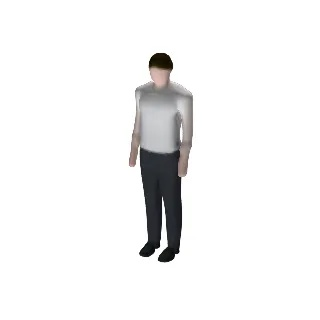
\includegraphics[width=0.25\linewidth]{images/supplementary/failure_case_bad/person_shap_e_r1c1.jpg} &
    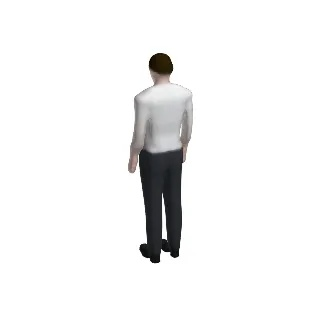
\includegraphics[width=0.25\linewidth]{images/supplementary/failure_case_bad/person_shap_e_r2c1.jpg} &
    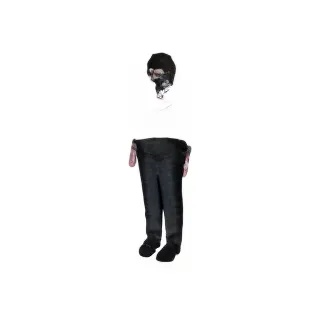
\includegraphics[width=0.25\linewidth]{images/supplementary/failure_case_bad/person_sharp_e_r1c1.jpg} &
    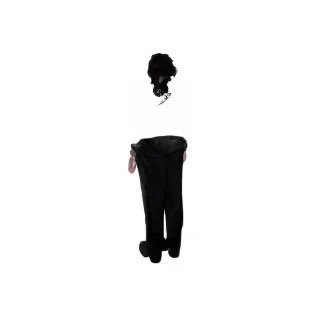
\includegraphics[width=0.25\linewidth]{images/supplementary/failure_case_bad/person_sharp_e_r2c1.jpg} \\
\end{tabular}
\caption{
A failure case of shap-e generation, Prompt: a man wearing a suit
}

\end{figure}
\section{Dataset Construction Details}

To construct our training dataset, we first encode high-quality 3D objects into Shap-E's latent space and render them under diverse lighting conditions (Figure~\ref{fig:multiple_lighting_conditions}). This ensures dataset variability, improving model robustness.

% \begin{figure}[htb]
%   \centering
%   \includegraphics[width=1\textwidth]{figures/multiple_lighting_conditions.png}
%   \caption{Objects rendered under multiple HDR lighting conditions to enrich the dataset.}
%   \label{fig:multiple_lighting_conditions}
% \end{figure}

We further apply filtering steps to maintain dataset quality. First, objects with significant geometric distortions or missing details, such as large white areas, are discarded (Figure~\ref{fig:filter_size_whitespace}). Secondly, we filter out semantically trivial or undesirable objects using their associated textual descriptions (Figure~\ref{fig:filter_text}).

% \begin{figure}[htb]
%   \centering
%   \includegraphics[width=1\textwidth]{figures/filter_size_whitespace.png}
%   \caption{Examples of objects filtered due to geometric distortions or excessive whitespace.}
%   \label{fig:filter_size_whitespace}
% \end{figure}

% \begin{figure}[htb]
%   \centering
%   \includegraphics[width=1\textwidth]{figures/filter_text_trading_cards.png}
%   \caption{Examples of semantically trivial objects filtered by text (e.g., trading cards).}
%   \label{fig:filter_text}
% \end{figure}

Additional examples illustrating the quality of the encode-decode process used to generate training pairs from Objaverse are shown in Figure~\ref{fig:dataset_encode_decode}.

% \begin{figure}[htb]
%     \centering
%     \includegraphics[width=1\textwidth]{figures/suplementary_encode_decode.png}
%     \caption{Encode-decode examples used for dataset generation. Left: original high-quality models. Right: degraded Shap-E encodings.}
%     \label{fig:dataset_encode_decode}
% \end{figure}

\section{Software and Resources}

All software developed during this research—including the Sharp-It model, dataset generation scripts, and visualization tools—will be made publicly available to support further academic and practical exploration. Relevant links, detailed instructions, and the source code repository accompany this thesis submission.